% Created by tikzDevice version 0.10.1 on 2017-12-03 20:41:17
% !TEX encoding = UTF-8 Unicode
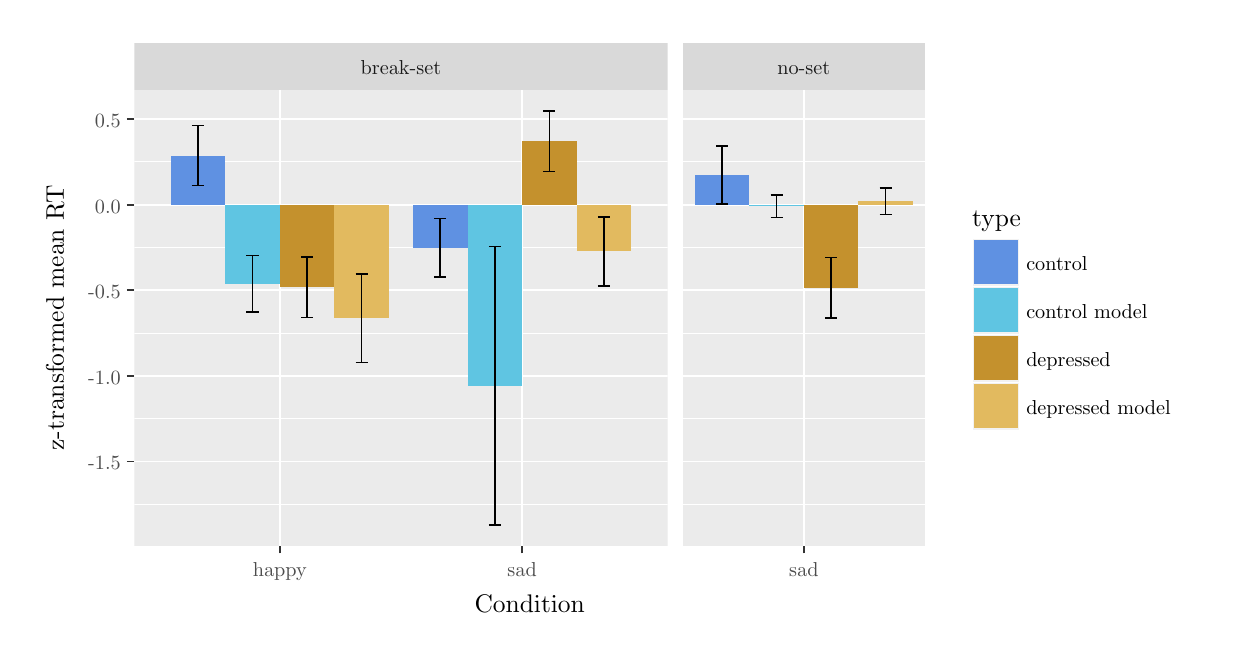
\begin{tikzpicture}[x=1pt,y=1pt]
\definecolor{fillColor}{RGB}{255,255,255}
\path[use as bounding box,fill=fillColor,fill opacity=0.00] (0,0) rectangle (433.62,216.81);
\begin{scope}
\path[clip] (  0.00,  0.00) rectangle (433.62,216.81);
\definecolor{drawColor}{RGB}{255,255,255}
\definecolor{fillColor}{RGB}{255,255,255}

\path[draw=drawColor,line width= 0.6pt,line join=round,line cap=round,fill=fillColor] ( -0.00,  0.00) rectangle (433.62,216.81);
\end{scope}
\begin{scope}
\path[clip] ( 38.57, 29.59) rectangle (231.20,194.25);
\definecolor{fillColor}{gray}{0.92}

\path[fill=fillColor] ( 38.57, 29.59) rectangle (231.20,194.25);
\definecolor{drawColor}{RGB}{255,255,255}

\path[draw=drawColor,line width= 0.3pt,line join=round] ( 38.57, 44.57) --
	(231.20, 44.57);

\path[draw=drawColor,line width= 0.3pt,line join=round] ( 38.57, 75.50) --
	(231.20, 75.50);

\path[draw=drawColor,line width= 0.3pt,line join=round] ( 38.57,106.43) --
	(231.20,106.43);

\path[draw=drawColor,line width= 0.3pt,line join=round] ( 38.57,137.36) --
	(231.20,137.36);

\path[draw=drawColor,line width= 0.3pt,line join=round] ( 38.57,168.30) --
	(231.20,168.30);

\path[draw=drawColor,line width= 0.6pt,line join=round] ( 38.57, 60.03) --
	(231.20, 60.03);

\path[draw=drawColor,line width= 0.6pt,line join=round] ( 38.57, 90.97) --
	(231.20, 90.97);

\path[draw=drawColor,line width= 0.6pt,line join=round] ( 38.57,121.90) --
	(231.20,121.90);

\path[draw=drawColor,line width= 0.6pt,line join=round] ( 38.57,152.83) --
	(231.20,152.83);

\path[draw=drawColor,line width= 0.6pt,line join=round] ( 38.57,183.76) --
	(231.20,183.76);

\path[draw=drawColor,line width= 0.6pt,line join=round] ( 91.11, 29.59) --
	( 91.11,194.25);

\path[draw=drawColor,line width= 0.6pt,line join=round] (178.66, 29.59) --
	(178.66,194.25);
\definecolor{fillColor}{RGB}{226,186,95}

\path[fill=fillColor] (110.81,111.85) rectangle (130.51,152.83);
\definecolor{fillColor}{RGB}{196,145,45}

\path[fill=fillColor] ( 91.11,123.00) rectangle (110.81,152.83);
\definecolor{fillColor}{RGB}{95,197,226}

\path[fill=fillColor] ( 71.40,124.24) rectangle ( 91.11,152.83);
\definecolor{fillColor}{RGB}{95,145,226}

\path[fill=fillColor] ( 51.70,152.83) rectangle ( 71.40,170.59);
\definecolor{fillColor}{RGB}{226,186,95}

\path[fill=fillColor] (198.36,135.99) rectangle (218.06,152.83);
\definecolor{fillColor}{RGB}{196,145,45}

\path[fill=fillColor] (178.66,152.83) rectangle (198.36,175.78);
\definecolor{fillColor}{RGB}{95,197,226}

\path[fill=fillColor] (158.96, 87.38) rectangle (178.66,152.83);
\definecolor{fillColor}{RGB}{95,145,226}

\path[fill=fillColor] (139.26,137.25) rectangle (158.96,152.83);
\definecolor{drawColor}{RGB}{0,0,0}

\path[draw=drawColor,line width= 0.6pt,line join=round] (118.47,127.86) --
	(122.84,127.86);

\path[draw=drawColor,line width= 0.6pt,line join=round] (120.66,127.86) --
	(120.66, 95.85);

\path[draw=drawColor,line width= 0.6pt,line join=round] (118.47, 95.85) --
	(122.84, 95.85);

\path[draw=drawColor,line width= 0.6pt,line join=round] ( 98.77,133.98) --
	(103.14,133.98);

\path[draw=drawColor,line width= 0.6pt,line join=round] (100.96,133.98) --
	(100.96,112.02);

\path[draw=drawColor,line width= 0.6pt,line join=round] ( 98.77,112.02) --
	(103.14,112.02);

\path[draw=drawColor,line width= 0.6pt,line join=round] ( 79.07,134.49) --
	( 83.44,134.49);

\path[draw=drawColor,line width= 0.6pt,line join=round] ( 81.26,134.49) --
	( 81.26,113.99);

\path[draw=drawColor,line width= 0.6pt,line join=round] ( 79.07,113.99) --
	( 83.44,113.99);

\path[draw=drawColor,line width= 0.6pt,line join=round] ( 59.37,181.43) --
	( 63.74,181.43);

\path[draw=drawColor,line width= 0.6pt,line join=round] ( 61.55,181.43) --
	( 61.55,159.74);

\path[draw=drawColor,line width= 0.6pt,line join=round] ( 59.37,159.74) --
	( 63.74,159.74);

\path[draw=drawColor,line width= 0.6pt,line join=round] (206.02,148.49) --
	(210.40,148.49);

\path[draw=drawColor,line width= 0.6pt,line join=round] (208.21,148.49) --
	(208.21,123.48);

\path[draw=drawColor,line width= 0.6pt,line join=round] (206.02,123.48) --
	(210.40,123.48);

\path[draw=drawColor,line width= 0.6pt,line join=round] (186.32,186.76) --
	(190.70,186.76);

\path[draw=drawColor,line width= 0.6pt,line join=round] (188.51,186.76) --
	(188.51,164.80);

\path[draw=drawColor,line width= 0.6pt,line join=round] (186.32,164.80) --
	(190.70,164.80);

\path[draw=drawColor,line width= 0.6pt,line join=round] (166.62,137.68) --
	(171.00,137.68);

\path[draw=drawColor,line width= 0.6pt,line join=round] (168.81,137.68) --
	(168.81, 37.07);

\path[draw=drawColor,line width= 0.6pt,line join=round] (166.62, 37.07) --
	(171.00, 37.07);

\path[draw=drawColor,line width= 0.6pt,line join=round] (146.92,147.82) --
	(151.30,147.82);

\path[draw=drawColor,line width= 0.6pt,line join=round] (149.11,147.82) --
	(149.11,126.69);

\path[draw=drawColor,line width= 0.6pt,line join=round] (146.92,126.69) --
	(151.30,126.69);
\end{scope}
\begin{scope}
\path[clip] (236.70, 29.59) rectangle (324.25,194.25);
\definecolor{fillColor}{gray}{0.92}

\path[fill=fillColor] (236.70, 29.59) rectangle (324.25,194.25);
\definecolor{drawColor}{RGB}{255,255,255}

\path[draw=drawColor,line width= 0.3pt,line join=round] (236.70, 44.57) --
	(324.25, 44.57);

\path[draw=drawColor,line width= 0.3pt,line join=round] (236.70, 75.50) --
	(324.25, 75.50);

\path[draw=drawColor,line width= 0.3pt,line join=round] (236.70,106.43) --
	(324.25,106.43);

\path[draw=drawColor,line width= 0.3pt,line join=round] (236.70,137.36) --
	(324.25,137.36);

\path[draw=drawColor,line width= 0.3pt,line join=round] (236.70,168.30) --
	(324.25,168.30);

\path[draw=drawColor,line width= 0.6pt,line join=round] (236.70, 60.03) --
	(324.25, 60.03);

\path[draw=drawColor,line width= 0.6pt,line join=round] (236.70, 90.97) --
	(324.25, 90.97);

\path[draw=drawColor,line width= 0.6pt,line join=round] (236.70,121.90) --
	(324.25,121.90);

\path[draw=drawColor,line width= 0.6pt,line join=round] (236.70,152.83) --
	(324.25,152.83);

\path[draw=drawColor,line width= 0.6pt,line join=round] (236.70,183.76) --
	(324.25,183.76);

\path[draw=drawColor,line width= 0.6pt,line join=round] (280.47, 29.59) --
	(280.47,194.25);
\definecolor{fillColor}{RGB}{226,186,95}

\path[fill=fillColor] (300.17,152.83) rectangle (319.88,154.04);
\definecolor{fillColor}{RGB}{196,145,45}

\path[fill=fillColor] (280.47,122.79) rectangle (300.17,152.83);
\definecolor{fillColor}{RGB}{95,197,226}

\path[fill=fillColor] (260.77,152.27) rectangle (280.47,152.83);
\definecolor{fillColor}{RGB}{95,145,226}

\path[fill=fillColor] (241.07,152.83) rectangle (260.77,163.57);
\definecolor{drawColor}{RGB}{0,0,0}

\path[draw=drawColor,line width= 0.6pt,line join=round] (307.84,158.76) --
	(312.21,158.76);

\path[draw=drawColor,line width= 0.6pt,line join=round] (310.03,158.76) --
	(310.03,149.33);

\path[draw=drawColor,line width= 0.6pt,line join=round] (307.84,149.33) --
	(312.21,149.33);

\path[draw=drawColor,line width= 0.6pt,line join=round] (288.14,133.74) --
	(292.51,133.74);

\path[draw=drawColor,line width= 0.6pt,line join=round] (290.32,133.74) --
	(290.32,111.84);

\path[draw=drawColor,line width= 0.6pt,line join=round] (288.14,111.84) --
	(292.51,111.84);

\path[draw=drawColor,line width= 0.6pt,line join=round] (268.44,156.29) --
	(272.81,156.29);

\path[draw=drawColor,line width= 0.6pt,line join=round] (270.62,156.29) --
	(270.62,148.24);

\path[draw=drawColor,line width= 0.6pt,line join=round] (268.44,148.24) --
	(272.81,148.24);

\path[draw=drawColor,line width= 0.6pt,line join=round] (248.74,174.13) --
	(253.11,174.13);

\path[draw=drawColor,line width= 0.6pt,line join=round] (250.92,174.13) --
	(250.92,153.01);

\path[draw=drawColor,line width= 0.6pt,line join=round] (248.74,153.01) --
	(253.11,153.01);
\end{scope}
\begin{scope}
\path[clip] ( 38.57,194.25) rectangle (231.20,211.31);
\definecolor{fillColor}{gray}{0.85}

\path[fill=fillColor] ( 38.57,194.25) rectangle (231.20,211.31);
\definecolor{drawColor}{gray}{0.10}

\node[text=drawColor,anchor=base,inner sep=0pt, outer sep=0pt, scale=  0.73] at (134.88,199.75) {break-set};
\end{scope}
\begin{scope}
\path[clip] (236.70,194.25) rectangle (324.25,211.31);
\definecolor{fillColor}{gray}{0.85}

\path[fill=fillColor] (236.70,194.25) rectangle (324.25,211.31);
\definecolor{drawColor}{gray}{0.10}

\node[text=drawColor,anchor=base,inner sep=0pt, outer sep=0pt, scale=  0.73] at (280.47,199.75) {no-set};
\end{scope}
\begin{scope}
\path[clip] (  0.00,  0.00) rectangle (433.62,216.81);
\definecolor{drawColor}{gray}{0.20}

\path[draw=drawColor,line width= 0.6pt,line join=round] ( 91.11, 26.84) --
	( 91.11, 29.59);

\path[draw=drawColor,line width= 0.6pt,line join=round] (178.66, 26.84) --
	(178.66, 29.59);
\end{scope}
\begin{scope}
\path[clip] (  0.00,  0.00) rectangle (433.62,216.81);
\definecolor{drawColor}{gray}{0.30}

\node[text=drawColor,anchor=base,inner sep=0pt, outer sep=0pt, scale=  0.73] at ( 91.11, 18.58) {happy};

\node[text=drawColor,anchor=base,inner sep=0pt, outer sep=0pt, scale=  0.73] at (178.66, 18.58) {sad};
\end{scope}
\begin{scope}
\path[clip] (  0.00,  0.00) rectangle (433.62,216.81);
\definecolor{drawColor}{gray}{0.20}

\path[draw=drawColor,line width= 0.6pt,line join=round] (280.47, 26.84) --
	(280.47, 29.59);
\end{scope}
\begin{scope}
\path[clip] (  0.00,  0.00) rectangle (433.62,216.81);
\definecolor{drawColor}{gray}{0.30}

\node[text=drawColor,anchor=base,inner sep=0pt, outer sep=0pt, scale=  0.73] at (280.47, 18.58) {sad};
\end{scope}
\begin{scope}
\path[clip] (  0.00,  0.00) rectangle (433.62,216.81);
\definecolor{drawColor}{gray}{0.30}

\node[text=drawColor,anchor=base east,inner sep=0pt, outer sep=0pt, scale=  0.73] at ( 33.62, 57.00) {-1.5};

\node[text=drawColor,anchor=base east,inner sep=0pt, outer sep=0pt, scale=  0.73] at ( 33.62, 87.94) {-1.0};

\node[text=drawColor,anchor=base east,inner sep=0pt, outer sep=0pt, scale=  0.73] at ( 33.62,118.87) {-0.5};

\node[text=drawColor,anchor=base east,inner sep=0pt, outer sep=0pt, scale=  0.73] at ( 33.62,149.80) {0.0};

\node[text=drawColor,anchor=base east,inner sep=0pt, outer sep=0pt, scale=  0.73] at ( 33.62,180.73) {0.5};
\end{scope}
\begin{scope}
\path[clip] (  0.00,  0.00) rectangle (433.62,216.81);
\definecolor{drawColor}{gray}{0.20}

\path[draw=drawColor,line width= 0.6pt,line join=round] ( 35.82, 60.03) --
	( 38.57, 60.03);

\path[draw=drawColor,line width= 0.6pt,line join=round] ( 35.82, 90.97) --
	( 38.57, 90.97);

\path[draw=drawColor,line width= 0.6pt,line join=round] ( 35.82,121.90) --
	( 38.57,121.90);

\path[draw=drawColor,line width= 0.6pt,line join=round] ( 35.82,152.83) --
	( 38.57,152.83);

\path[draw=drawColor,line width= 0.6pt,line join=round] ( 35.82,183.76) --
	( 38.57,183.76);
\end{scope}
\begin{scope}
\path[clip] (  0.00,  0.00) rectangle (433.62,216.81);
\definecolor{drawColor}{RGB}{0,0,0}

\node[text=drawColor,anchor=base,inner sep=0pt, outer sep=0pt, scale=  0.92] at (181.41,  5.50) {Condition};
\end{scope}
\begin{scope}
\path[clip] (  0.00,  0.00) rectangle (433.62,216.81);
\definecolor{drawColor}{RGB}{0,0,0}

\node[text=drawColor,rotate= 90.00,anchor=base,inner sep=0pt, outer sep=0pt, scale=  0.92] at ( 13.08,111.92) {z-transformed mean RT};
\end{scope}
\begin{scope}
\path[clip] (  0.00,  0.00) rectangle (433.62,216.81);
\definecolor{fillColor}{RGB}{255,255,255}

\path[fill=fillColor] (335.63, 65.58) rectangle (428.12,158.25);
\end{scope}
\begin{scope}
\path[clip] (  0.00,  0.00) rectangle (433.62,216.81);
\definecolor{drawColor}{RGB}{0,0,0}

\node[text=drawColor,anchor=base west,inner sep=0pt, outer sep=0pt, scale=  0.92] at (341.32,144.99) {type};
\end{scope}
\begin{scope}
\path[clip] (  0.00,  0.00) rectangle (433.62,216.81);
\definecolor{drawColor}{RGB}{255,255,255}
\definecolor{fillColor}{gray}{0.95}

\path[draw=drawColor,line width= 0.6pt,line join=round,line cap=round,fill=fillColor] (341.32,123.31) rectangle (358.67,140.65);
\end{scope}
\begin{scope}
\path[clip] (  0.00,  0.00) rectangle (433.62,216.81);
\definecolor{fillColor}{RGB}{95,145,226}

\path[fill=fillColor] (342.04,124.02) rectangle (357.96,139.94);
\end{scope}
\begin{scope}
\path[clip] (  0.00,  0.00) rectangle (433.62,216.81);
\definecolor{drawColor}{RGB}{255,255,255}
\definecolor{fillColor}{gray}{0.95}

\path[draw=drawColor,line width= 0.6pt,line join=round,line cap=round,fill=fillColor] (341.32,105.96) rectangle (358.67,123.31);
\end{scope}
\begin{scope}
\path[clip] (  0.00,  0.00) rectangle (433.62,216.81);
\definecolor{fillColor}{RGB}{95,197,226}

\path[fill=fillColor] (342.04,106.67) rectangle (357.96,122.60);
\end{scope}
\begin{scope}
\path[clip] (  0.00,  0.00) rectangle (433.62,216.81);
\definecolor{drawColor}{RGB}{255,255,255}
\definecolor{fillColor}{gray}{0.95}

\path[draw=drawColor,line width= 0.6pt,line join=round,line cap=round,fill=fillColor] (341.32, 88.62) rectangle (358.67,105.96);
\end{scope}
\begin{scope}
\path[clip] (  0.00,  0.00) rectangle (433.62,216.81);
\definecolor{fillColor}{RGB}{196,145,45}

\path[fill=fillColor] (342.04, 89.33) rectangle (357.96,105.25);
\end{scope}
\begin{scope}
\path[clip] (  0.00,  0.00) rectangle (433.62,216.81);
\definecolor{drawColor}{RGB}{255,255,255}
\definecolor{fillColor}{gray}{0.95}

\path[draw=drawColor,line width= 0.6pt,line join=round,line cap=round,fill=fillColor] (341.32, 71.27) rectangle (358.67, 88.62);
\end{scope}
\begin{scope}
\path[clip] (  0.00,  0.00) rectangle (433.62,216.81);
\definecolor{fillColor}{RGB}{226,186,95}

\path[fill=fillColor] (342.04, 71.98) rectangle (357.96, 87.91);
\end{scope}
\begin{scope}
\path[clip] (  0.00,  0.00) rectangle (433.62,216.81);
\definecolor{drawColor}{RGB}{0,0,0}

\node[text=drawColor,anchor=base west,inner sep=0pt, outer sep=0pt, scale=  0.73] at (360.84,128.95) {control};
\end{scope}
\begin{scope}
\path[clip] (  0.00,  0.00) rectangle (433.62,216.81);
\definecolor{drawColor}{RGB}{0,0,0}

\node[text=drawColor,anchor=base west,inner sep=0pt, outer sep=0pt, scale=  0.73] at (360.84,111.60) {control model};
\end{scope}
\begin{scope}
\path[clip] (  0.00,  0.00) rectangle (433.62,216.81);
\definecolor{drawColor}{RGB}{0,0,0}

\node[text=drawColor,anchor=base west,inner sep=0pt, outer sep=0pt, scale=  0.73] at (360.84, 94.26) {depressed};
\end{scope}
\begin{scope}
\path[clip] (  0.00,  0.00) rectangle (433.62,216.81);
\definecolor{drawColor}{RGB}{0,0,0}

\node[text=drawColor,anchor=base west,inner sep=0pt, outer sep=0pt, scale=  0.73] at (360.84, 76.91) {depressed model};
\end{scope}
\end{tikzpicture}
